\begin{center}
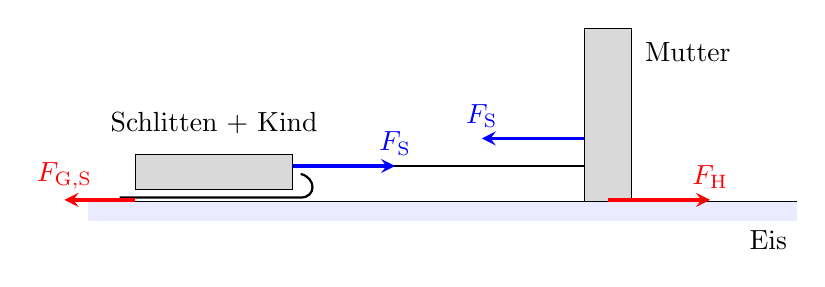
\begin{tikzpicture}[>=stealth]
 \fill[blue!8] (-5,0) rectangle (4,-0.25);
 \draw (-5,0) -- (4,0);
 \node[anchor=north east] at (4,-0.25) {Eis};
 \draw[fill=gray!30] (-4.4,0.15) rectangle (-2.4,0.6);
 \draw[thick] (-4.6,0.05) -- (-2.3,0.05) .. controls (-2.1,0.05) and (-2.1,0.3) .. (-2.3,0.35);
 \node at (-3.4,1.0) {Schlitten + Kind};
 \draw[fill=gray!30] (1.3,0) rectangle (1.9,2.2);
 \node[anchor=west] at (1.95,1.9) {Mutter};
 \draw[thick] (-2.4,0.45) -- (1.3,0.45);
 \draw[->, very thick, blue] (-2.4,0.45) -- ++(1.3,0) node[above] {$F_\mathrm{S}$};
 \draw[->, very thick, red] (-4.4,0.02) -- ++(-0.9,0) node[above] {$F_\mathrm{G,S}$};
 \draw[->, very thick, blue] (1.3,0.8) -- ++(-1.3,0) node[above] {$F_\mathrm{S}$};
 \draw[->, very thick, red] (1.6,0.02) -- ++(1.3,0) node[above] {$F_\mathrm{H}$};
\end{tikzpicture}
\end{center}

Wir nehmen an, dass die Mutter den Schlitten mit horizontalem Seil gleichförmig zieht. Am Schlitten ist die Seilkraft dann gleich der Gleitreibungskraft der Stahlkufen auf dem Eis, $\mu_\mathrm{G} = \muGO$ (FoTaBe S.~189):
\begin{align}
 F_\mathrm{S} &= \mu_\mathrm{G}\,m_\mathrm{S}\,g
\end{align}
Das Seil zieht die Mutter mit derselben Kraft nach hinten. Sie bleibt nur dann im Gleichgewicht, wenn die Haftreibungskraft des Eises auf ihre Sohlen diese Kraft aufbringen kann:
\begin{align}
 \mu_\mathrm{G}\,m_\mathrm{S}\,g &\leq \mu_\mathrm{H}\,m_\mathrm{M}\,g
\end{align}
Die Masse von Kind und Schlitten darf also höchstens
\begin{align}
 m_\mathrm{S} &= \mSlF \\
   &= \frac{\muH\cdot\mMu}{\muG} \\
   &= \mSl \approx \result{\mSlP{0}{2}}
\end{align}
betragen. Um den ruhenden Schlitten anzuziehen, muss die Haftreibung der Kufen ($\mu_\mathrm{H,S} = \muSHO$) überwunden werden; das gelingt nur bis $m_\mathrm{S} = \mShP{0}{2}$.
